\documentclass[12pt]{report}

%==Commonly used packages==%
\usepackage{graphicx,subfig} %For Figures
%\usepackage{graphicx,subfigure} %For Figures
\usepackage{amsmath,amssymb,amsthm,array} %For mathematical symbols
\usepackage{tabularx}	% for tables
\usepackage{rotating, booktabs}  % For table-rotating 
\usepackage{tikz} %ploww
\usepackage[skip=8pt]{caption} %ploww, for vertical spcae between caption and fig
\usepackage{hyperref}


\usepackage{booktabs}
\usepackage[detect-all]{siunitx}
%\setlength{\parindent}{0pt}
\setlength\parskip{ \baselineskip}
%\usepackage{feynman}

\usepackage{multirow}
\usepackage{Thesis-defs} % definition
\usepackage{xspace}
%==========================%
%==Format of NTHU Thesis==%
\usepackage[a4paper, top=2.54cm, bottom=2.54cm, left=3.17cm, right=3.17cm]{geometry}  % This is the standard setting of thesis of NTHU. Do not change it.
\linespread{1.5}  % The linespread is 1.5.
\newtheorem{thm}{Theorem}[section]  % Define new theorem.
\newtheorem{alg}{Algorithm}[section]  % Define new algorithm.
\usepackage{wallpaper}  % For watermark
\CenterWallPaper{.18}{./Figures/nthu-logo}  % Watermark of NTHU
\theoremstyle{plain}
%=========================%
%====For Chinese typing=====%
\usepackage{xeCJK,fontspec} 
\setCJKmainfont{楷體-繁} 
\XeTeXlinebreaklocale "zh" 
\XeTeXlinebreakskip = 0pt plus 1pt
%===========================%
%====For Roman number====% 如果用不到羅馬數字可以註解掉
\makeatletter %define for Roman number
\newcommand{\rom}[1]{\romannumeral #1} %小寫羅馬數字1=rom{1}
\newcommand{\Rom}[1]{\expandafter\@slowromancap\romannumeral #1@} %大寫羅馬數字1=Rom{1}
%========================%
\setlength\@fptop{0\p@}
\makeatother




\begin{document}

\begin{titlepage}  % Titlepage 封面
\begin{center}
\Huge
\textbf{國立清華大學\\物理系\\碩士學位論文\\}
\vspace*{1.5in}
\huge
%\textbf{利用ATLAS偵測器探討由向量玻色子融合產生之希格斯玻色子衰變至W玻色子對與其之WW背景估計}
	
\textbf{利用ATLAS偵測器探討由向量玻色子融合產生希格斯玻色子之W玻色子對衰變與其WW背景估計}
	
%	量測WW背景在向量玻色子融合希格斯粒子\\同步化的數值研究\\}
\LARGE
\textbf{Estimation of the WW background in the Vector Boson Fusion H$\rightarrow$WW$^{(*)}$ Analysis with the ATLAS
Detector\\}
%\vspace*{1in} 
\vfill
%\Large $\:$校$\:$ $\:$ $\:$名$\,$ ($\:$系$\:$ $\:$ $\:$所$\,$):國立清華大學\\
\Large 系所組別:物理所物理組\\
\Large 學號姓名: 106022504 蔡孟儒 (Meng-Ju Tsai)\\
%\Large $\:$作$\:$ $\:$ $\:$者$\,$:蔡孟儒 Meng-Ju Tsai\\
%\Large $\:$學$\:$ $\:$ $\:$號$\,$:106022504\\
\Large $\:$$\:$$\,$指導教授$\,$:徐百嫻$\,$教授 (Prof. Pai-Hsien Hsu)$\:$\\ 
%\vspace*{0.5in} 
\vfill
\Large 中$\,$華$\,$民$\,$國$\,$一$\bigcirc$八$\,$年$\,$一$\,$月
\end{center}
\end{titlepage}

\begin{titlepage} %書名頁
\begin{center}
\huge {Estimation of the WW background in the Vector Boson Fusion H$\rightarrow$WW$^{(*)}$ Analysis with the ATLAS
	Detector\\}
\vspace*{1.5in}
\large A Thesis Presented to \\the Department of Physics at \\National Tsing Hua University \\in Partial Fulfillment for the Requirement of \\the Master of Science Degree Program\\
\vspace*{2in}
\large By\\Meng-Ju Tsai\\
\large Advisor\\Dr. Pai-Hsien Hsu\\
\large January 2019
\end{center}
\end{titlepage}
 %封面和書名頁
\begin{abstract}  % Abstract 
We present ....
\newpage  % Independent page
\thispagestyle{empty}
\begin{center}
\vspace*{1.2in}
\large 摘要\\
\end{center}
\normalsize
此論文探討 ...


\end{abstract}



 %中英文摘要
\begin{center}
\textbf{Acknowledgements}  % Acknowledgements
\end{center}
{\small
%\begin{CJK}{UTF8}{cwku}  % For Chinese typing
特別感謝 ...
\newpage %致謝
\pagenumbering{roman} %從這頁開始用羅馬頁碼
\tableofcontents  % Table of contents
\addcontentsline{toc}{chapter}{Contents}
\newpage
\listoftables  % List of tables
\addcontentsline{toc}{chapter}{List of Tables}
\listoffigures  % List of figures
\addcontentsline{toc}{chapter}{List of Figures}
\newpage %目錄和圖表
\pagenumbering{arabic} %從這頁開始用數字頁碼

\chapter{Introduction} 
%cite放在./Part/Reference,如果Thesis.tex第一次看到這個位置,他不知道要到下面去找,要編譯兩次才會出現引用編號。


%==================== Higgs ====================%
\section{The Discovery of the Higgs Boson}
The Higgs boson is discovered ..

\begin{figure}[!h]
	\graphicspath{ {./Figures/} }
	\centering
	\begin{minipage}[h]{0.45\textwidth}
		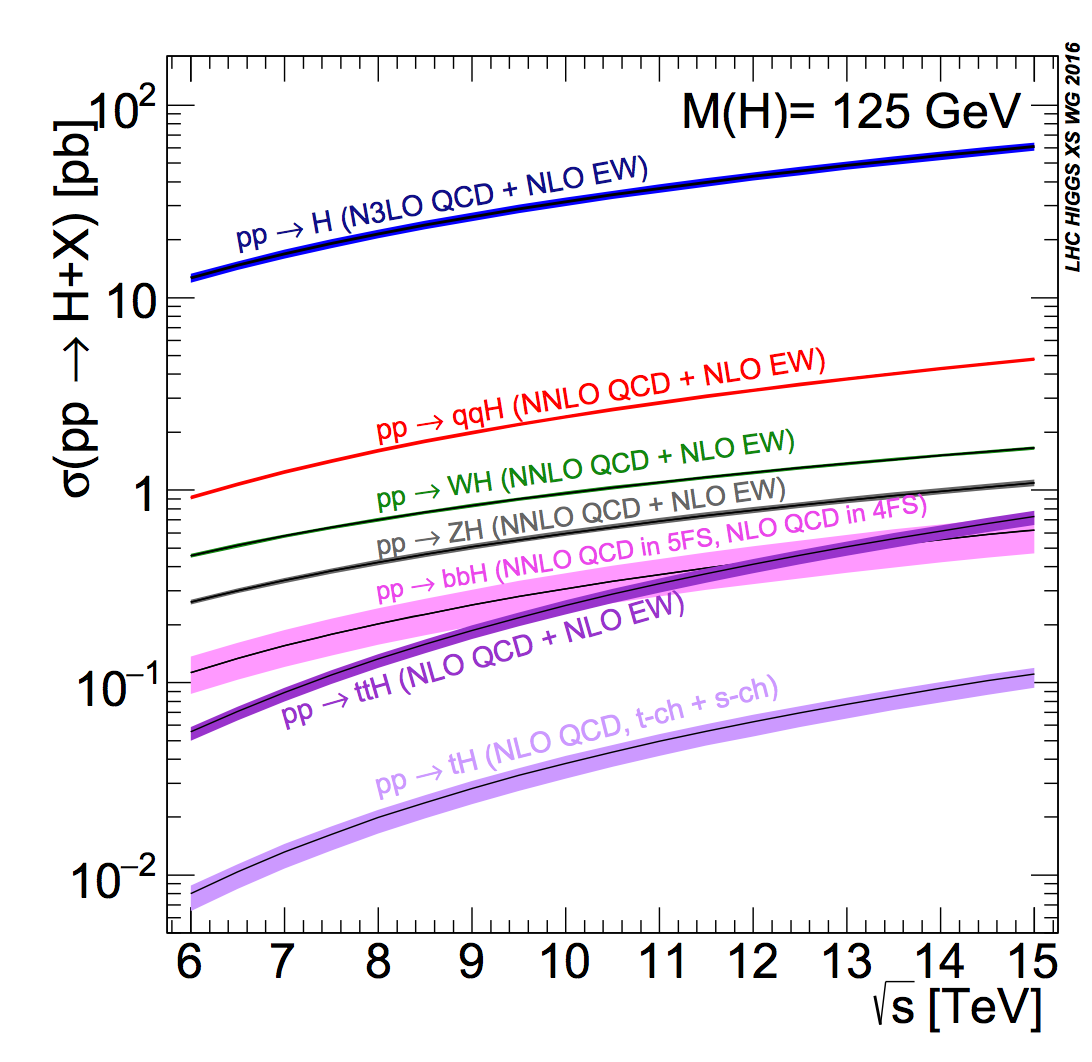
\includegraphics[width=1\linewidth]{/Introduction/Higgs/XsecHiggs}
	\end{minipage}
	\begin{minipage}[h]{0.54\textwidth}
		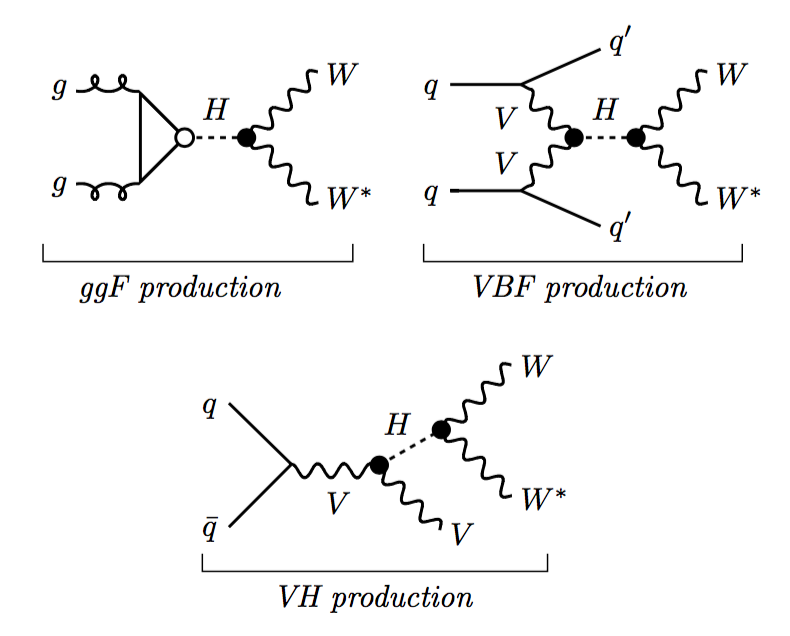
\includegraphics[width=1\linewidth]{/other/HIGGS_PRO}
	\end{minipage}
	\caption{Expected cross-sections of the productions of the Higgs bosons (left). The Feynman diagrams of the leading production modes of the Higgs boson which further decays to  $WW^{(*)}$ (right). Letter "V" represents a W or Z boson \cite{ATLAS:2014aga}.}
	\label{fig:Higgs_pro}
\end{figure}


\begin{figure}[!h]
	\graphicspath{ {./Figures/} }
	\centering
	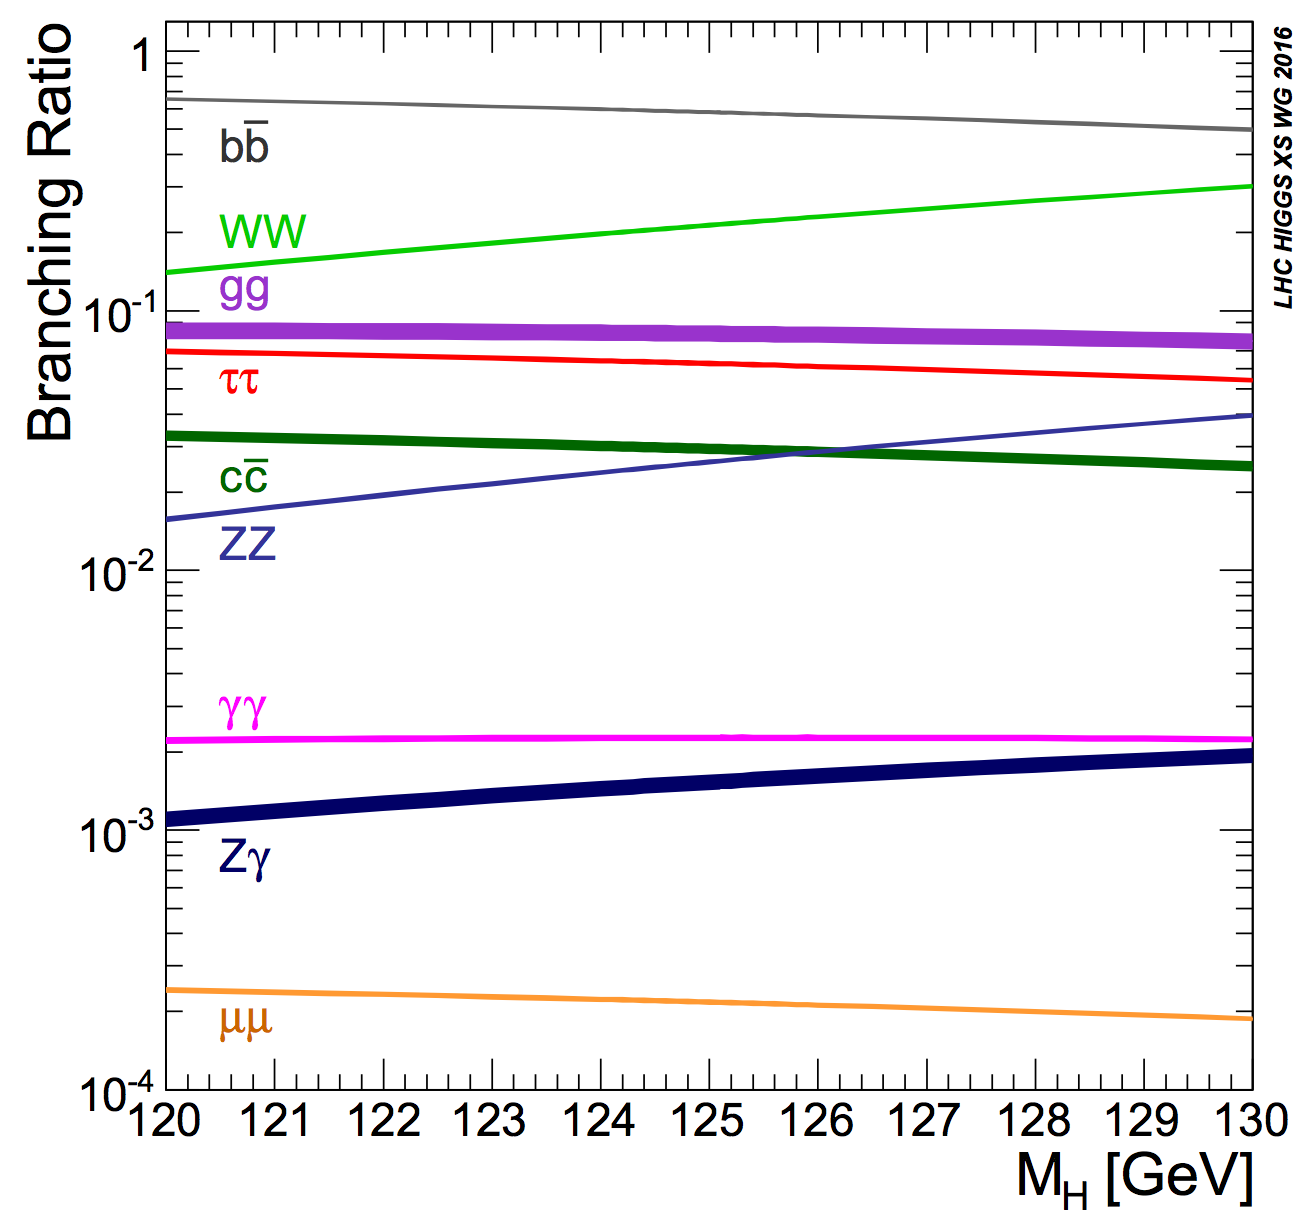
\includegraphics[width=0.5\linewidth]{/Introduction/Higgs/HiggsBR}
	\caption{Branching ratios of decays of Higgs bosons \cite{PDGReview}.}
	\label{fig:Higgs_decay}
\end{figure}





%==================== VBF HWW ====================%
 
\chapter{The ATLAS experiment}

\section{The ATLAS detector}

The ATLAS detector \cite{ATLAS:2014aga, Detector} is used for this analysis. ...

\begin{figure}
	\centering
	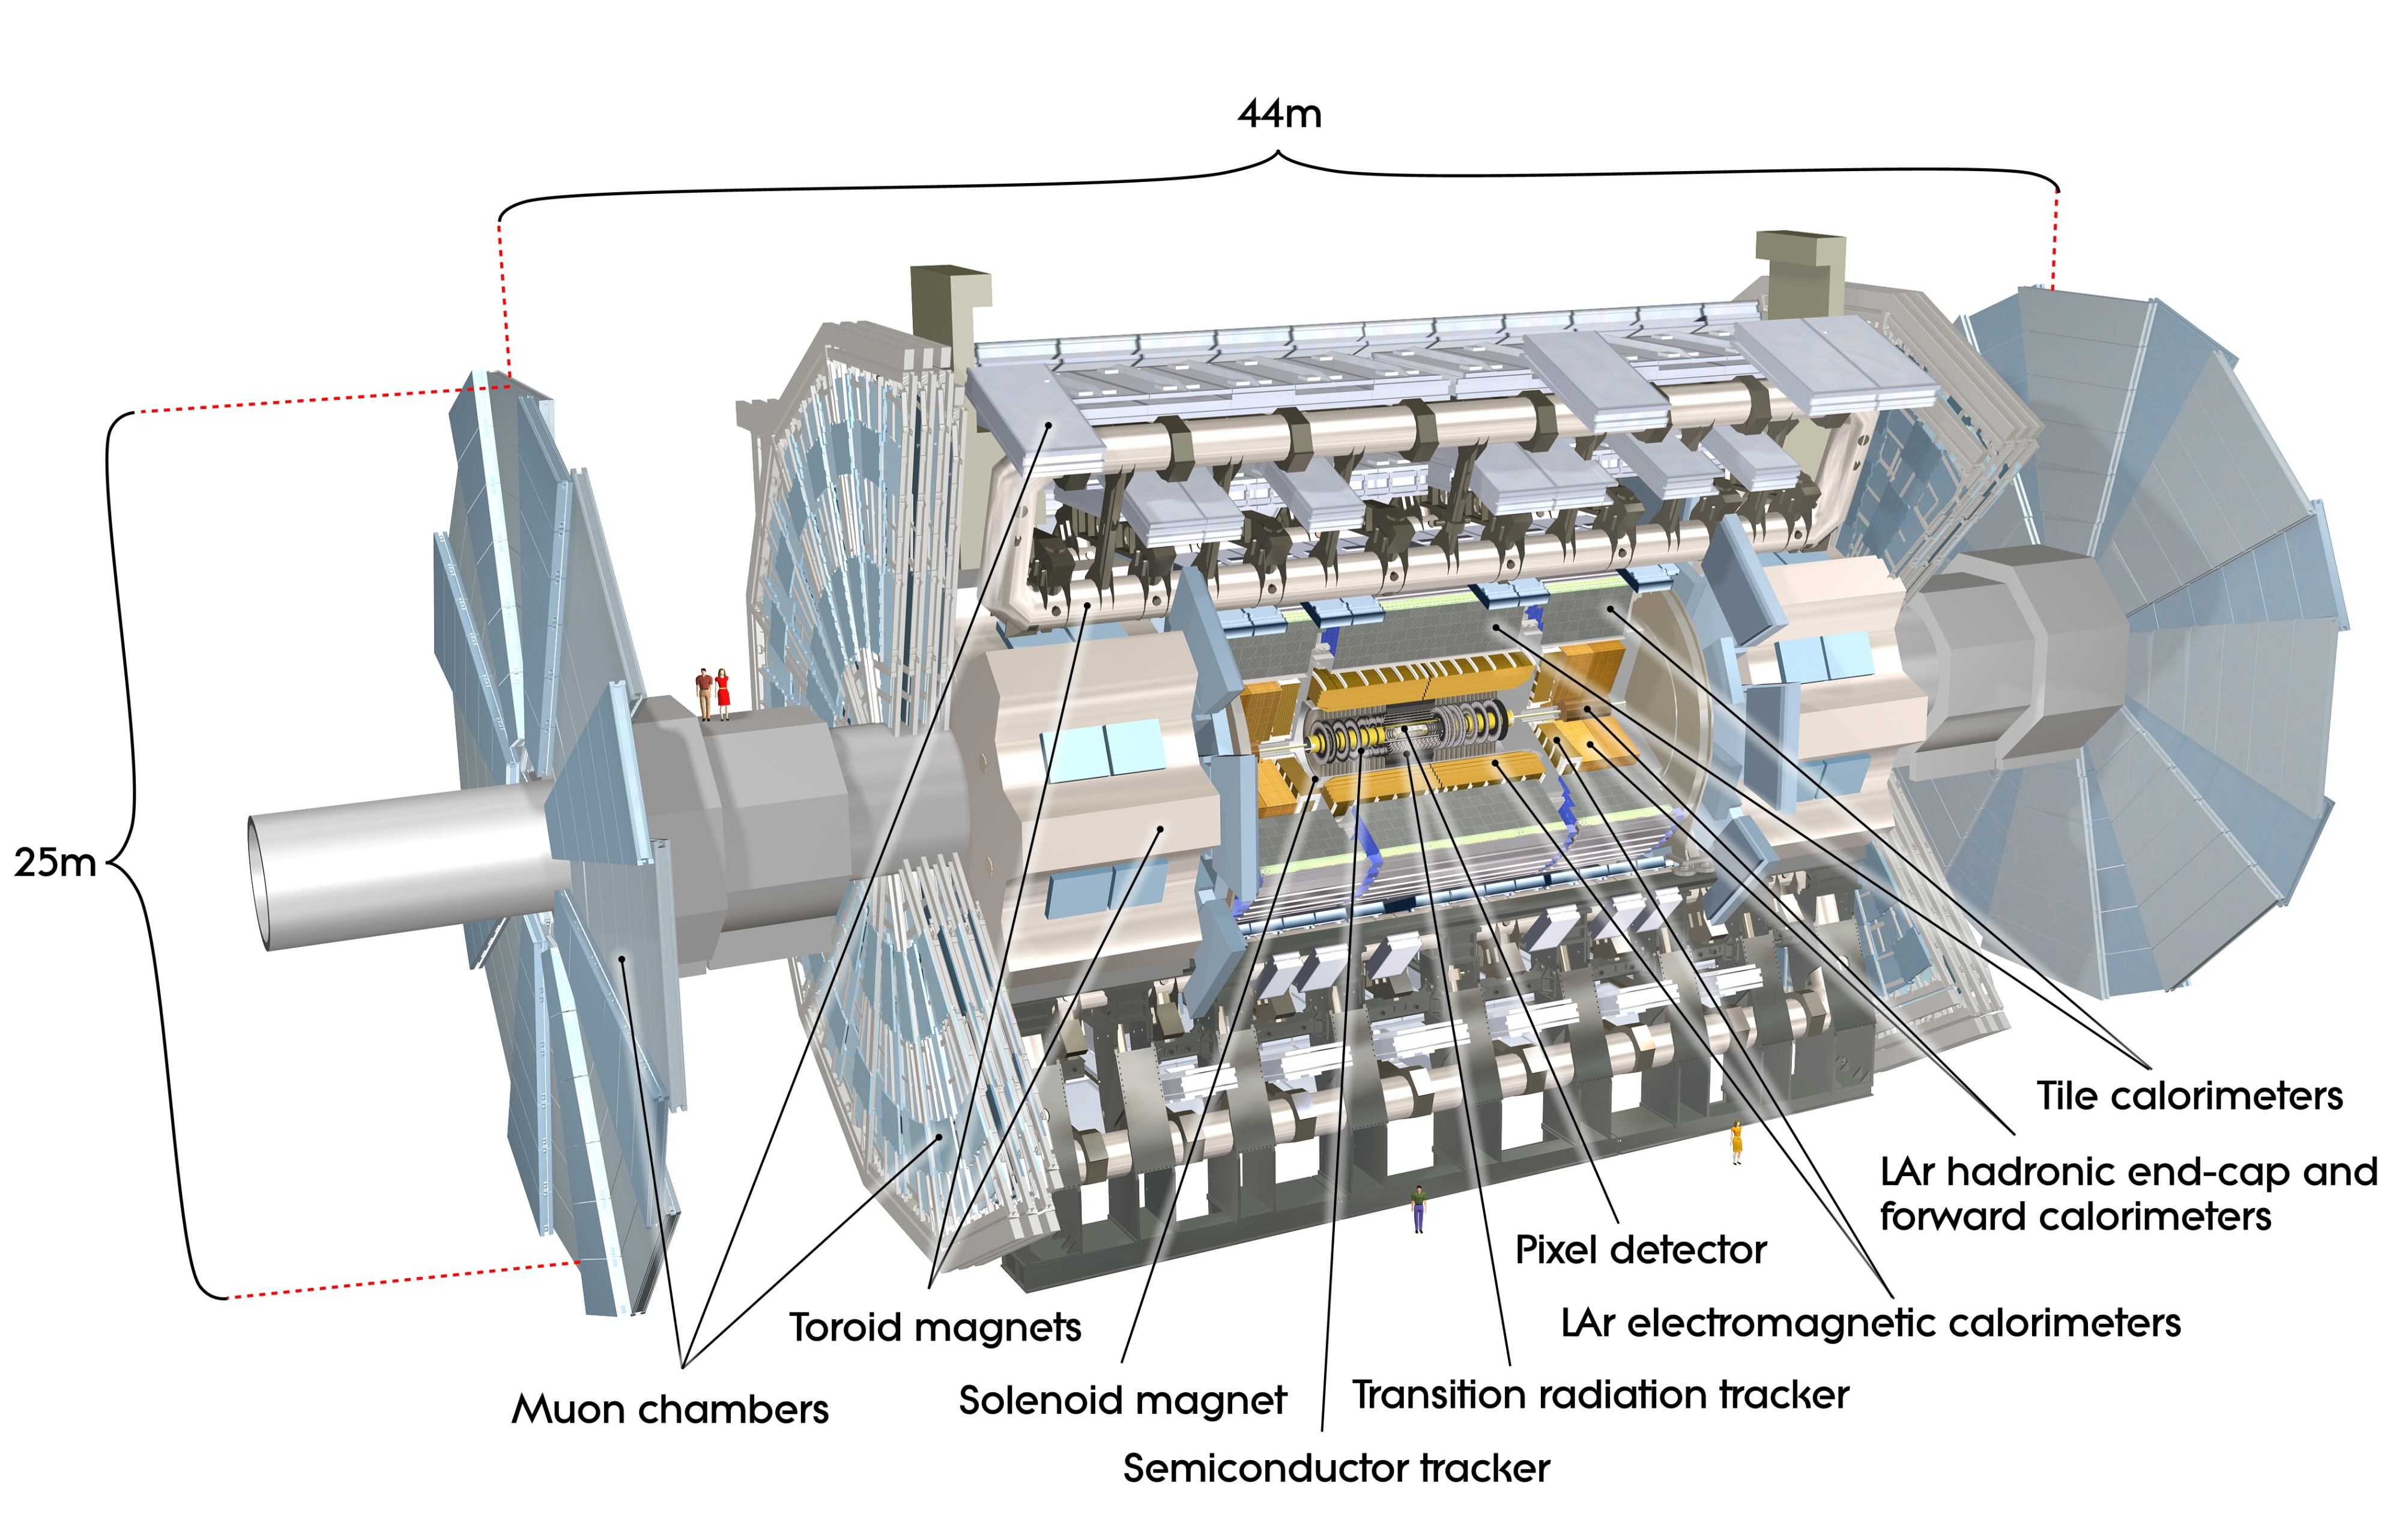
\includegraphics[width=0.8\linewidth]{Figures/ATLAS_detector}
	\caption{The structure of ATLAS detector \cite{Detector}.}
	\label{fig:ATLAS_detector}
\end{figure}
...


\section{Data and MC samples}

\subsection{Data samples}\label{subsec:data_trigger}
The data samples ...

\subsection{MC samples}\label{MCsamples}

...



\chapter{VBF \hwwlnln analysis}\label{section:VBFanalysis}

This chapter is organized as follow. Section \ref{VBF:CommonSelection} provides ...

%Section \ref{subsec:data_trigger} discusses the triggers used, the trigger efficiencies and the gains of signals with the current setup.
\section{Common event selection}\label{VBF:CommonSelection}
...

\begin{itemize}
	\item Exactly two opposite charged and different flavor leptons ($e\mu+\mu e$)
	\item $\pTlead > 22$ \gev, $\pTsublead > 15$ \gev
	\item $\mll > 10$ \gev
\end{itemize}




\section{Construction of the VBF  phase space}\label{VBF:VBFSR}

\subsection{Experimental signature of VBF Higgs boson}\label{VBF:Signature}
The VBF production is characterized ... 




\subsection{Event selection for VBF-enriched phase space}\label{VBF:EventSelection}

After the common event selection ...

\begin{table}[!h]
	\centering
	\caption{Ranking of the BDT training variables \cite{ATLASComNote}.}
	\label{tab:ranking}
	\scalebox{0.8}{
		\vspace{0.3cm}
\begin{tabular}{ c | c  | c }
\hline
\hline
Ranking & Variable & Importance [\%]\\
\hline
1       & $\mathrm{m_{jj}}$            & 19\\
2       & $\mathrm {\Delta y_{jj}}$    & zz\\
3       & $\mathrm {m_{ll}}$           & xx\\
4       & $m_T$                        & yy\\
5       & lepton $\eta$ centrality     & zz\\
6       & $\mathrm{\Delta \phi_{ll}}$  & aa\\
7       & $\mathrm{\sum_{l,j} M_{lj}}$ & bb \\
8       & $\mathrm{p^{T}_{tot}}$       & cc \\
\hline
\hline
\end{tabular}

	}
\end{table}


%\begin{figure}[t]
%	\begin{minipage}{0.5\textwidth}
%		\centering
%		\includegraphics[width=0.9\linewidth, angle=-90]{Figures/VBFAnalysis/BDTInput/emme-CutVBFbVeto_2jet-Mll-lin}
%	\end{minipage}
%	\begin{minipage}{0.5\textwidth}
%		\centering
%		\includegraphics[width=0.9\linewidth, angle=-90]{Figures/VBFAnalysis/BDTInput/emme-CutVBFbVeto_2jet-DPhill-lin}
%	\end{minipage}
%		\begin{minipage}{0.5\textwidth}
%			\centering
%			\includegraphics[width=0.9\linewidth, angle=-90]{Figures/VBFAnalysis/BDTInput/emme-CutVBFbVeto_2jet-DYjj-lin}
%		\end{minipage}
%			\begin{minipage}{0.5\textwidth}
%				\centering
%				\includegraphics[width=0.9\linewidth, angle=-90]{Figures/VBFAnalysis/BDTInput/emme-CutVBFbVeto_2jet-Mjj-lin}
%			\end{minipage}
%		\caption{Distributions of BDT inputs $\mll$, $\dphill$, $\dyjj$ and $\mjj$ after VBF pre-selection. The VBF signal is scaled by a factor of 300 \cite{ATLASComNote}.}
%		\label{fig:BDTinput1}
%	\end{figure}

\begin{table}[!h]
	\centering
	\caption{ 
		Event yields in the VBF SR after fitting. Event yields in the highest BDT bin are also presented. The uncertainties include systematic and statistical uncertainties \cite{HWWRun2Paper}.}
	\label{tab:ggF_VBF_yields}
	\scalebox{0.8}{
		\begin{tabular}{lS[table-format=4.1,table-number-alignment=right]@{$\,\pm\,$}
                     S[table-format=3.2,table-number-alignment=left]
                     S[table-format=4.2,table-number-alignment=right]@{$\,\pm\,$}
                     S[table-format=3,table-number-alignment=left]
                     S[table-format=2,table-number-alignment=right]@{$\,\pm\,$}
%                     S[table-format=4.1,table-number-alignment=left]
%                     S[table-format=3.3,table-number-alignment=right]@{$\,\pm\,$}
%                     S[table-format=2,table-number-alignment=left]
                     }
  \dbline
  Process  & \multicolumn{5}{c}{\TwoJet VBF}  \tabularnewline
             &  \multicolumn{2}{c}{Inclusive} &\multicolumn{3}{c}{BDT: $[0.86,1.0]$}\tabularnewline
  \sgline
  $H_{\mathrm{ggF}}$                   &  42   & 16 & 6   &  3   \tabularnewline
  $H_{\mathrm{VBF}}$                  &  xx   & yy & zz  &  xx   \tabularnewline
  \sgline                                               
  $WW$                                &  xx   & yy & zz  &  xx    \tabularnewline
  $VV$                           &  xx   & yy & zz  &  xx    \tabularnewline
  $t\bar{t}/Wt$                     &  xx   & yy & zz  &  xx     \tabularnewline
  Mis-Id                           &  xx   & yy & zz  &  xx    \tabularnewline
  $Z/\gamma^{*}$                &  xx   & yy & zz  &  xx     \tabularnewline
  \sgline
  Total                         &  xx   & yy & zz  &  xx    \tabularnewline
  Observed   &  \multicolumn{2}{l}{2164}  & \multicolumn{2}{l}{\quad60}  \tabularnewline
  \dbline
  \end{tabular}
 
	}
\end{table}


\begin{figure}[!h]
\centering
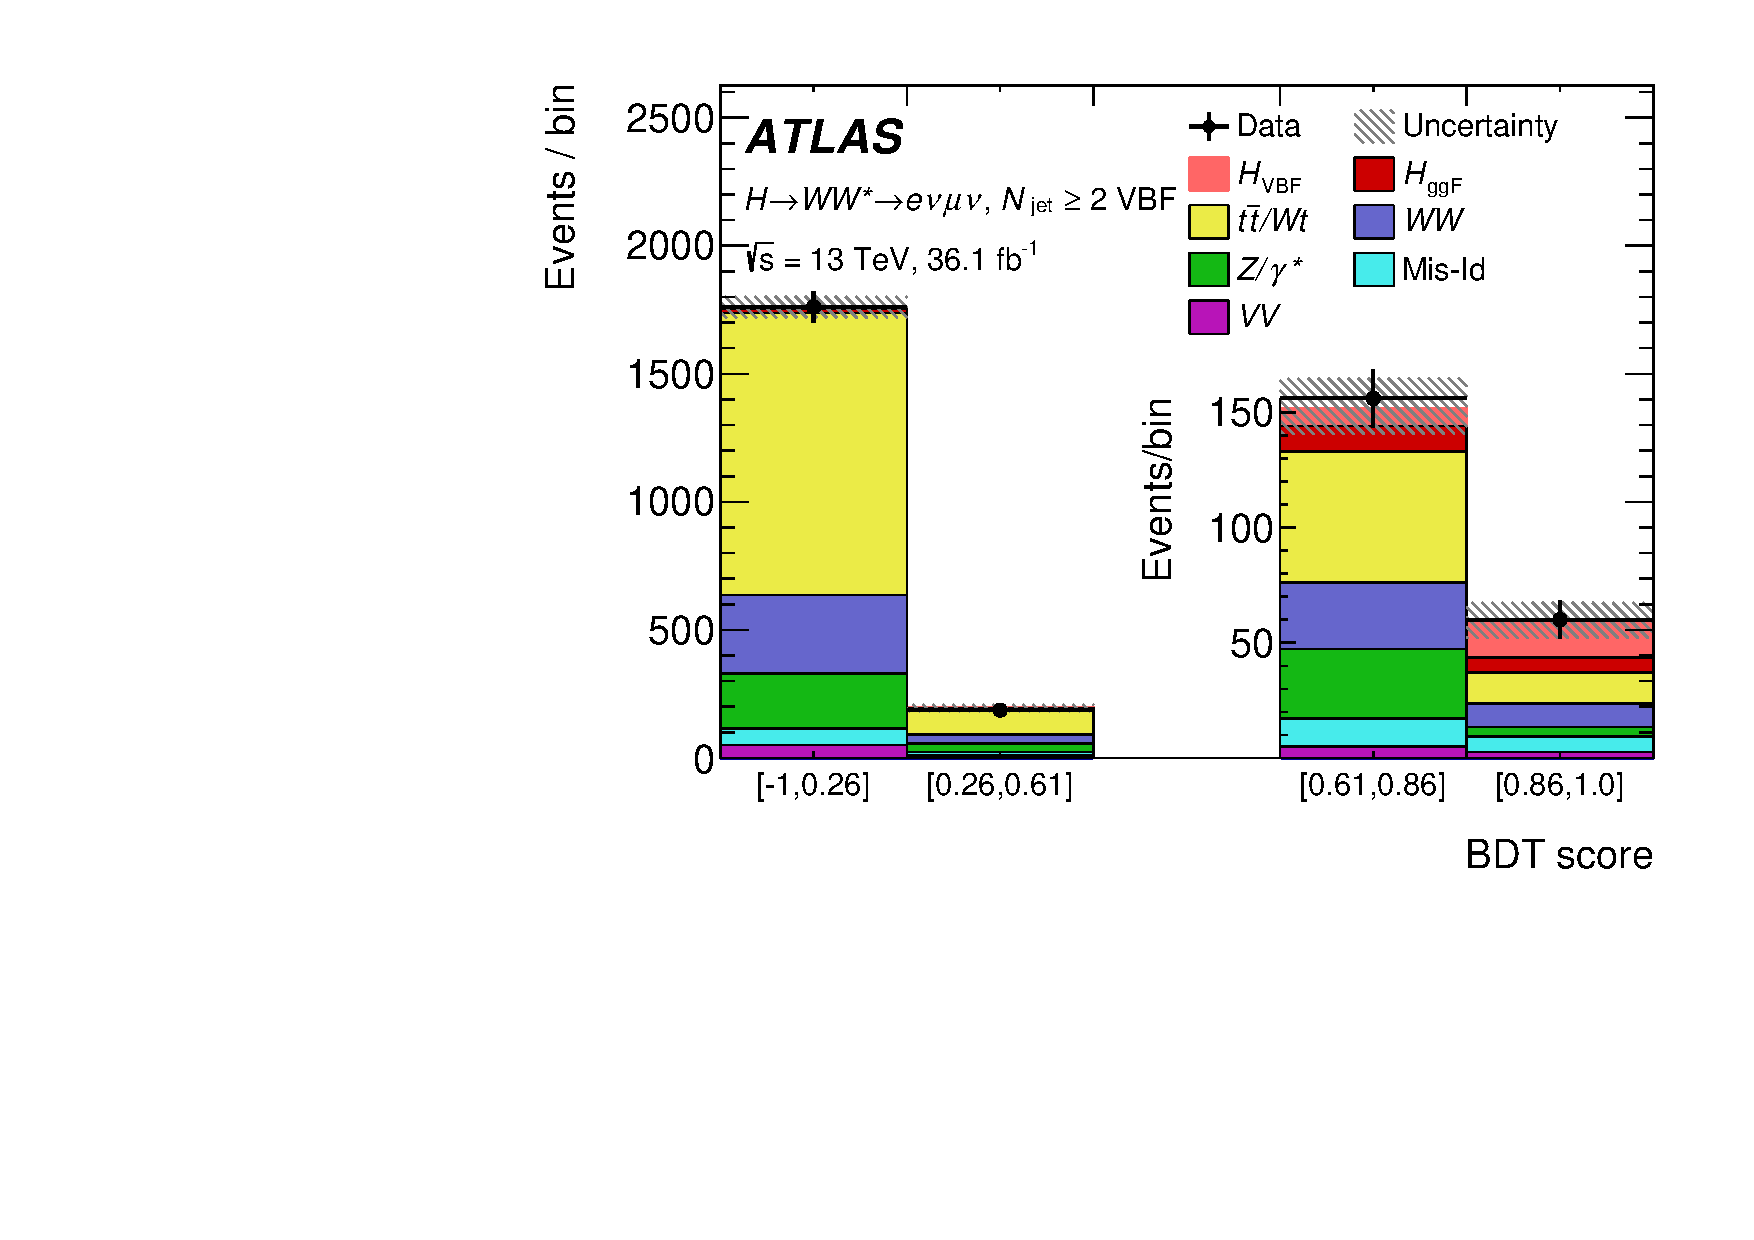
\includegraphics[width=0.45\linewidth, angle=-90]{Figures/VBFAnalysis/BDT_newStyle_V03}
\caption{Distribution of BDT scores in the VBF SR after fitting is shown. The hatched error band shows the total uncertainty of signal and background MC prediction \cite{HWWRun2Paper}.}
\label{fig:BDT_newStyle_V03}
\end{figure}

\section{Results of VBF analysis in Run-2}\label{VBF:Results}
The signal strength $\mu$ is the ratio of the measured signal yields to the signal yields predicted by the SM. The signal strength for VBF analysis in our final publication \cite{HWWRun2Paper} is shown below:

\begin{equation}
\mu_{\mathrm{VBF}} =  0.62^{+0.29}_{-0.27} (\mathrm{stat.})^{+0.12}_{-0.13} (\mathrm{theo~ syst.})\pm 0.15(\mathrm{exp~ syst.}) = 0.62^{+0.36}_{-0.35}.
\end{equation}\label{eqn:SignalStrength}


\chapter{The estimation of WW background} \label{EstWW:Main}

In this chapter, ...

\section{Normalization factor}\label{EstWW:intro}


\section{Construction of a WW CR}\label{EstWW:construction}



\subsection{$m_{T}$ and $m_{T2}$ variables}\label{EstWW:mtmt2}

\chapter{Conclusion and Outlook}

%\chapter{Outlook}\label{Outlook}

\addcontentsline{toc}{chapter}{Appendix}  % Add "Appendix" into the table of contents


\appendix
\chapter{Appendix}\label{app}

%\section{Data/MC comparison after $\mt > 130$ \gev}

\section{Event displays for Higgs boson candidates}\label{app:EvtDisplay}


\section{Re-estimation of WW theoretical uncertainties with the modified $\pTtot$ variable}\label{app:NewPttot}


\section{Optimization of the selections for VBF phase space}\label{app:OptVBFspace}



\pagebreak 
\begin{thebibliography}{99}
\addcontentsline{toc}{chapter}{Reference}  % Add "Reference" into the table of contents

\bibitem{ATLAS:Aad20121}The ATLAS Collaboration, {\it Observation of a new particle in the search for the Standard Model Higgs boson with the ATLAS detector at the LHC},  Phys. Lett. B B716 (2012) 1-29.
\bibitem{Chatrchyan:2012xdj}The CMS Collaboration, {\it Observation of a new boson at a mass of 125 GeV with the CMS experiment at the LHC}, Phys. Lett. B 716 (2012) 30.
\bibitem{ATLAS:2014aga}The ATLAS Collaboration, {\it Observation and measurement of Higgs boson decays to WW* with the ATLAS detector}, Phys. Rev. D 92, 012006 (2015).
\bibitem{LHCXsec}The LHC Higgs Cross Section Working Group, {\it Handbook of LHC Higgs Cross Sections: 3. Higgs Properties}, arXiv: 1307.1347.
\bibitem{PDGReview}M. Tanabashi et al. (Particle Data Group), {\it 2018 Review of Particle Physics}, Phys. Rev. D 98, 030001 (2018).
\bibitem{Detector}The ATLAS Collaboration, {\it The ATLAS Experiment at the CERN Large Hadron Collider}, JINST 3 (2008) S08003.
\bibitem{PID}Christian Lippmann, {\it Particle identification}, Nucl.Instrum.Meth. A666 (2012) 148-172.
\bibitem{ATLASComNote}Claudia Bertella et al., {\it Measurements of the Higgs boson production cross section via ggF and VBF in $H\rightarrow WW^{(*)} \rightarrow l\nu l\nu$ with 36.1 fb$^{−1}$ of data collected with the ATLAS detector at $\sqrt{s}$=13 TeV}, ATL-COM-PHYS-2017-1094.
\bibitem{HWWRun2Paper}The ATLAS Collaboration, {\it Measurements of gluon-gluon fusion and vector-boson fusion Higgs boson production cross-sections in the $\hwwlnln$ decay channel in pp collisions at $\com = $13 TeV with the ATLAS detector}, Phys. Lett. B 789 (2019) 508.

\end{thebibliography}
\newpage
 
\end{document}